\chapter{Distributed computing}
As mentioned, low scalability is a problem in a Siemens windmill farm. The Wind Power Supervisor (WPS) and the HPPP does not scale well with the number of turbines, which introduces performance issues to the solution. Both in terms handling external requests, which is done by the WPS, but also when regulating the windmill farm through the HPPP. 

An example of this is the HPPP regulation sequence illustrated on \cref{fig:dataComputationSequence}. Today this sequence takes approximately 150 ms. Siemens wishes this time reduced to 10 ms. This is a major performance improvement and for that reason, performing the regulation sequence using a distributed database only is not enough, since reading/writing to the disk decreases performance.

When distributing the Wind Power Supervisor onto the turbines, the turbines obviously needs to be able to handle these external requests and windmill farm regulations. For the heavy tasks, in terms of CPU power, distributed computing becomes relevant as a way of improving performance by combining the CPU power residing inside the turbines to compute a common task.

In distributed computing, each node or process has its own local memory and communication happens via message passing \cite{andrews2000foundations}. This chapter describes relevant distributed computing communication paradigms and discusses which technology that is the best for the Siemens case. 


\section{Message passing}

Message passing is a low-level communication paradigm, where processors communicate by sending messages via bidirectional channels. It's a highly used paradigm and other communication paradigms are usually implemented on top of an underlying message-passing system.  

With message passing being a low-level communication paradigm, the communication overhead is low compared to paradigms build on top of it. It is entirely up to the application developer to handle communication. This will in many cases result in better performance, which is the most compelling argument for choosing message passing as communication paradigm. The problem with it being up to the developer, is that the developer needs to deal with configurations setup, exception handling, who and when to communicate with, etc., when developing the application. This makes it hard to develop using message passing, compared to distributed shared memory, especially when dealing with more complex applications \cite{lu1995message}. 


\section{Distributed shared memory}

Shared memory is an attractive paradigm for designing parallel and distributed systems. Applications can use shared memory as a tool for the entire system to share a common state. However for loose coupled distributed systems, no physically shared memory is available to support such a model. Distributed shared memory (DSM) is a way of providing physically distributed memory machines a shared memory abstraction, illustrated on \cref{fig:distributedSharedMemory}.

\begin{figure}
	\centering
	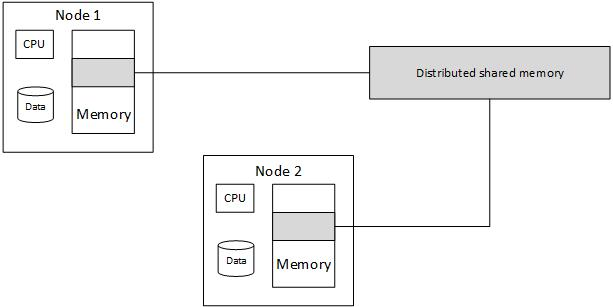
\includegraphics[width=0.8\textwidth,natwidth=610,natheight=642]{DistributedSharedMemory.jpg} 
	\captionsetup{format=plain,font=footnotesize,labelfont={bf,defaultCapFont},labelsep=quad,singlelinecheck=no}
	\caption[Distributed Computing System with 2 nodes]{
		\label{fig:distributedSharedMemory} 
		\footnotesize{%
			A distributed shared memory system with 2 nodes.
		}
	}
\end{figure}

The primary advantage of DSM over message passing is the shared memory abstraction provided. This gives the illusion of physically shared memory and allows developers to use the shared-memory paradigm, without having to think about communication mechanisms. However the abstraction also introduces overhead to the system, which decreases performance. The DSM abstraction has limited knowledge of the application flow of the application, compared to communication via message passing. 
 
Comparing DSM with message passing with regards to performance is not entirely fair since DSM is build on top of message passing. However the comparison is necessary when considering what technology to use for a given system and in this case, the comparison results in a trade off between performance and the shared memory abstraction. 

Honghui \cite{lu1995message} has studied the trade-off between message passing performance and the shared memory abstraction. He ported 12 different parallel program scenarios to a DSM system called TreadMarks and a message passing system called PVM and compared the two technologies with regards to programmability and performance. He argues that given DSM is an abstraction built on top of message passing, DSM cannot achieve better performance than message passing, given the larger software-overhead. Therefore the goal is to achieve the same performance as message passing using DSM. For 5 of the scenarios, TreadMarks performed within 10\% of PVM. For 6 of the programs the difference were between 10\% - 30\%. For the last scenario, PVM performed twice as well as TreadMarks. 

Honghui argues that the performance is dependent of the logical flow of the scenario. More messages and more data are sent in TreadMarks, explaining the performance differences. He gives the following reasons for the extra communication in TreadMarks:

\begin{itemize}
	\item Separation of synchronization and data transfer in TreadMarks. 
	\item Extra messages to request updates for data in the invalidate protocol used in TreadMarks.
	\item False sharing.
	\item Diff accumulation for migratory data in TreadMarks.
\end{itemize} 

%1) Seperation of synchronization
% Lazy release consistency: Against data races (which may result uin wrong results). Only the next processor that acquires the lock can access x --> only that processor is informormed of the change to x --> reduce message traffic. Ex: Barriers - No processor overites values before all processors have read the value computed in the previous interation.

%2) Extra messages to request updates for data in the invalidate protocol used in TreadMarks
% Memory page change communicatin. Modified pages are inviladated after an acquire. Later access causes access miss, which in turn causes installation of an up-to-date copy of the page.

%3) False sharing
% To objects er allokerede i samme memory page og de skrives til samtidig --> force update af page --> overhead

%4) diff accumulation for migratory data in TreadMarks
% Multiple-writer protocol to allow wrinting on same page at the same time. Uses a diff algorithm to reduce false sharing effects.

Honghui concludes that the performance of a well optimized DSM system is comparable to that of a message passing system. Furthermore, development of systems with complex communication patterns takes a lot less effort using the DSM paradigm.

In contrast to Honghui, Stumm and Zhou \cite{stumm1990algorithms} argues that applications using DSM can in fact outperform their message passing counterparts, in a few cases. They argue, that this is possible for the following reasons:

\begin{itemize}
 	\item DSM algorithms typically move data on demand as they are being accessed, which spreads communication load over a longer period of time, allowing for a greater degree of concurrency. If for example a node uses the shared memory more than others, the node does not need to communicate for every write operation made to the shared memory.
 	\item For DSM algorithms that sends data in large blocks, communication overhead is reduced. 
\end{itemize} 
 

%DSM pass by reference

%In distribted system there might be scenarios in which a task waits for a service at the queue of one resource, while at the same time another resource which is capable of serving the task is idle. The purpose of a load balancing algorithm is to prevent these scenarios as much as possible.

%three phases.
%Information collection: Gathers info of workload
%decision making: Calc optimal data dist.
%data migration: Transfer excess amount of workload from on overloaded processor to another underloaded processor

%Centralized: Size of grid increases, keppeing all the inforation about the state of all the resources is a bottlebeck. Scalability becomes an issue. Page 281. 

%The benifits of this technique stems from Load Balancing
%State Broadcast Algorithm (SBA). Page 282

%Basic assumptions Page 289.

%Scalability and makespan (Y). Page 298, conclusion.


\section{Publish/subscribe}

Publish/subscribe is a messaging pattern where communication is interest based instead of address based. Messages are characterized into classes and sent by publishers, without knowledge of how many subscribers there may be. Nodes can then subscribe to one or more classes of interest, without knowledge of how many publishers there are, providing a more decoupled, scalable and flexible interaction model.

\begin{figure}
	\centering
	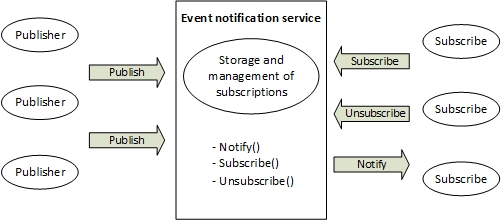
\includegraphics[width=0.9\textwidth,natwidth=610,natheight=642]{PublishSubscribe.jpg} 
	\captionsetup{format=plain,font=footnotesize,labelfont={bf,defaultCapFont},labelsep=quad,singlelinecheck=no}
	\caption[Distributed Computing System with 2 nodes]{
		\label{fig:publishSubscribe} 
		\footnotesize{%
			A simple publish/subscribe system.
		}
	}
\end{figure}

The publish/subscribe paradigm is event driven. The paradigm relies on an event notification service providing storage and management for subscriptions and efficient delivery of events, as illustrated on \cref{fig:publishSubscribe} \cite{eugster2003many}. The subscribers are notified subsequently of any event, generated by a publisher, matching the registered interest. The strength of this event-based communication is the full decoupling in time, space and synchronization between publishers and subscribers \cite{eugster2003many}.




\section{Remote message invocation}


\section{Conclusion}

%Ens
%Valg med vægt på arkitektur og development tid. 
%RMI fravalg